\documentclass[11pt]{article}
    \title{\textbf{Maths IA - Written 1}}
    \date{}
    \author{Jack Larkin}
    \usepackage{graphicx}
	\graphicspath{ {./} }
    \addtolength{\topmargin}{-3cm}
    \addtolength{\textheight}{3cm}
\begin{document}

\maketitle

\section*{Algebra}
\subsection*{(a)}
Since \textbf{X} is a solution to the linear system, the unkown values can be found via simple substitution and algebra. After substituting \textbf{x}, the system becomes:
$$3(1) + 3(0) - 2 + w = 0$$
$$-4(0) + 2(2) + t(w) = 0$$
And then:
$$3-2+w=0$$
$$4+t(w)=0$$
From which it can be shown that $w=-1$, and consequently that $t=4$.
\\\\\textbf{Answer:} $w=-1,t=4$.
\subsection*{(b)}
As any solution to a linear system will also be a solution to an equivalent linear system, this question too can be answered via substituting \textbf{X} into the linear system as follows:
$$1 + 0 - 2 -1 = 0$$
$$3(1)-0+2+5(-1)=0$$
If and only if \textbf{both} of these equations can be shown to be true, then the linear system could equivalent, however, looking at the first equation in the system, it's clear that $1+0-2-1=-2\neq 0$. Even though the second equation can be said to be sound, this is enough to claim that the two systems are not equivalent.
 \\\\\textbf{Answer:} Not Equivalent.
 \\\\\\\\
\section*{Calculus}
\subsection*{(a)}
The graph of $f(n)=p_n$, where $p_n$ is the number of primes in the prime factorisation of of $n$, is shown below over the resticted domain $\{1,2,...,12\}$.
\begin{figure}[h]
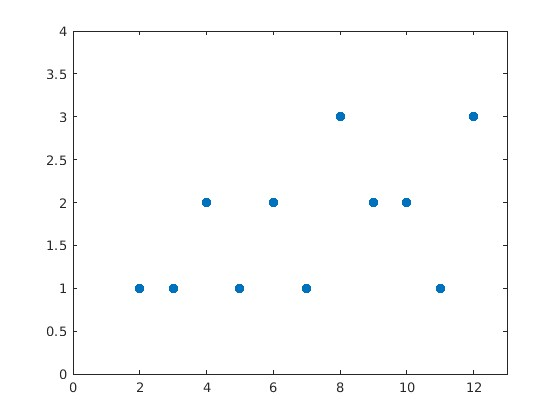
\includegraphics[scale=0.7]{primefactorgraph}
\centering
\end{figure}
\\The values for $f(n)$ were found by manually computing the prime factorisation of each integer in the domain and are as follows:
$$f(2)=1,\;f(3)=1,\;f(4)=2,\;f(5)=1,\;f(6)=2,\;f(7)=1$$
$$f(8)=3,\;f(9)=2,\;f(10=2,\;f(11)=1,\;f(12)=3$$
\subsection*{(b)}
$f$ is not one to one, as it can be easily demonstrated that for two values such that $n_1\neq n_2$, $f(n_1)=f(n_2)$. Indeed, for the graph in question (a), it requires nothing more than observation to notice that while $2\neq 3\neq 5\neq 7\neq 11$, it is the case that $f(2)=f(3)=f(5)=f(7)=f(11)$. Therefore, the function is clearly not one-to-one, as it fails the horizontal line test (more than once!).
\\\\\textbf{Answer:} Not one-to-one 
\subsection*{(c)}
To show why the range of $f$ is equal to $\mathbf{N}$, it needs to be demonstrated that $f(n)=m,\;m \in \mathbf{N}$.
\\\\First, express $n$ differently such that $n = 2^m,\; n,m \in \mathbf{N}$, and notice that the prime factorisation of any number $2^m$ will look like $2\times 2\times ...\times 2$, $m$ times. Ergo, $f(2^m) = m$, where $m$ can be any natural number. Therefore $f(n)$ can take any value in the set of natural numbers, and the range of $f$ is equal to $\mathbf{N}$. 
\end{document}

